\documentclass[10pt,a4paper,final,twocolumn]{article}

\usepackage{algorithm}
\usepackage{algpseudocode}
\usepackage{amssymb}
\usepackage[english]{babel}
\usepackage{color}
\usepackage[colorlinks=false,%
            pdfkeywords={},%
            pdftitle={Fast garbage compaction with interior pointers},%
            pdfauthor={Benedikt Meurer},%
            pdfsubject={},%
            pdfdisplaydoctitle=true]{hyperref}
\usepackage{tikz}

\usetikzlibrary{arrows}
\usetikzlibrary{decorations.pathreplacing}

\begin{document}

\author{%
  Benedikt Meurer\\
  Compilerbau und Softwareanalyse\\
  Universit\"at Siegen\\
  D-57068 Siegen, Germany\\
  \url{meurer@informatik.uni-siegen.de}
}
\date{}
\title{
  Fast garbage compaction with interior pointers
}
\maketitle

\begin{abstract}
  This paper presents a garbage compaction algorithm, which extends the well-known
  algorithm of Jonkers with the ability to handle interior pointers. It is as efficient
  as Jonkers' algorithm in the absence of interior pointers, and in practice only
  slightly less efficient in the presence of interior pointers, while at the same
  time, it does not impose any additional space overhead. This, however, is partly due
  to the fact that only certain kinds of interior pointers are allowed.
\end{abstract}


\section{Introduction}
\label{sec:Introduction}


Compacting garbage collection is a useful technique to implement heap storage management
in modern runtime environments. The need for compaction of heap storage and a growing
number of compaction techniques have been presented previously.

Today there are basically two classes of compaction algorithms. The first class employs a
new area as large as the original heap area and compact
the heap by moving live block to a contiguous segment of the new area. Algorithms in
this class are usually referred to as \emph{copying garbage collectors} or \emph{semi-space
garbage collectors} \cite{Cheney70,Clark76,FenichelYochelson69,Minsky63,Reingold73}.

The other class generally
traces and marks all storage in use, plan where the live blocks of storage are to be
moved, update each pointer to point to the planned address of the referenced block, and
finally move each block to its planned address. Algorithms in this class are usually
referred to as \emph{mark-compact garbage collectors}
\cite{Fisher74,FitchNorman78,HaddonWaite67,Jonkers79,LangWegbreit72,Morris78,Thorelli76,Wegbreit72}.

This paper deals with the well-known compaction algorithm presented by Jonkers \cite{Jonkers79},
which compacts live blocks within a single contiguous heap space by sliding them to the low end
of the heap space. This algorithm is one of the most popular garbage compactors because it requires
only two heap passes, does not impose any additional space overhead and is relatively easy to
adapt. However -- in its basic form -- it cannot cope with pointers to the interior of live blocks.

We will present an extension to the basic algorithm, which adds support for pointers containing
addresses of special interior cells, called \emph{interior header cells}. We start by defining the
problem in section~\ref{sec:problem}. Section~\ref{sec:jonkers} describes the basic algorithm.
Then, in section~\ref{sec:our}, we present our extended algorithm. Section~\ref{sec:efficiency}
reviews the efficiency of the extended algorithm. Finally section~\ref{sec:related} compares our
work with related compaction algorithms.


\section{Problem}
\label{sec:problem}


Following the original problem statement in \cite{Jonkers79} we represent a machine memory
by an array $M$ of \emph{cells}. Every cell has a unique \emph{address}, which is the index
of the cell in $M$. A \emph{pointer} is an address or the special value $\mathbf{nil}$, which
is not equal to any address in $M$. We assume that each cell is large enough to contain a
pointer.

There is a subarray $S$ of $M$ with indices $s_1,\ldots,s_k$, called the \emph{store}, which is
the part of $M$ to be compacted.
The store $S$ contains a number of disjoint subarrays called \emph{nodes}. Every node contains
exactly one \emph{header cell}, zero or more \emph{interior header cells} and a number of
\emph{pointer cells}, which are cells that contain a pointer. The \emph{header address} of a
node is the address of its header cell. An \emph{interior address} of a node is the address
of one of its interior header cells. Every node thereby has one or more \emph{addresses},
formed by the \emph{header address} and the \emph{interior addresses}.
For the sake of simplicity we take the first cell of a node to be the
header cell.

We assume that the contents of the header and interior header cells are distinguishable from
a pointer. Furthermore we assume that a pointer $q$ in a pointer cell of a node is
either $\mathbf{nil}$ or points to a node, i.e. $q$ is either $\mathbf{nil}$ or an
address of a node.

Just before the call to the compaction routine, the marking phase of the garbage collector
will have established the following information:
\begin{enumerate}
\item The addresses $r_1,\ldots,r_n$ of cells not contained in $S$, which contain either
  $\mathbf{nil}$ or a pointer to a node. These addresses are called \emph{root set} and
  form the starting points of the marking phase.
\item The header addresses $l_1,\ldots,l_m$ of the nodes contained in $S$. These nodes have been
  determined by the marking phase as being \emph{live} (i.e. non-garbage).
\end{enumerate}
This situation is schematically shown in Fig.~\ref{fig:Machine_memory_after_marking_phase}.

\begin{figure}[htb]
  \centering
  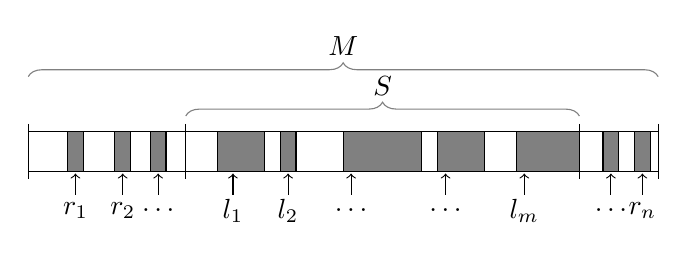
\begin{tikzpicture}
    \draw (0,1) rectangle (8,0.5);
    \draw (0.0,1.1) -- (0.0,0.4);
    \draw (8,1.1) -- (8,0.4);
    \draw [gray,decorate,decoration={brace,amplitude=5pt}] (0,1.7) -- (8,1.7) node [black,midway,above=4pt] {$M$};
    %% Root set start r_1,...
    \filldraw [fill=gray] (0.5,1) rectangle (0.7,0.5);
    \draw [->] (0.6,0.2) -- (0.6,0.47);
    \draw (0.6,0) node {$r_1$};
    \filldraw [fill=gray] (1.1,1) rectangle (1.3,0.5);
    \draw [->] (1.2,0.2) -- (1.2,0.47);
    \draw (1.2,0) node {$r_2$};
    \filldraw [fill=gray] (1.55,1) rectangle (1.75,0.5);
    \draw [->] (1.65,0.2) -- (1.65,0.47);
    \draw (1.65,0) node {$\ldots$};
    %% store S
    \draw (2,1.1) -- (2,0.4);
    \draw (7,1.1) -- (7,0.4);
    \draw [gray,decorate,decoration={brace,amplitude=5pt}] (2.0,1.2) -- (7,1.2) node [black,midway,above=4pt] {$S$};
    \filldraw [fill=gray] (2.4,1) rectangle (3.0,0.5);
    \draw [->] (2.6,0.2) -- (2.6,0.47);
    \draw (2.6,0) node {$l_1$};
    \filldraw [fill=gray] (3.2,1) rectangle (3.4,0.5);
    \draw [->] (3.3,0.2) -- (3.3,0.47);
    \draw (3.3,0) node {$l_2$};
    \filldraw [fill=gray] (4.0,1) rectangle (5.0,0.5);
    \draw [->] (4.1,0.2) -- (4.1,0.47);
    \draw (4.1,0) node {$\ldots$};
    \filldraw [fill=gray] (5.2,1) rectangle (5.8,0.5);
    \draw [->] (5.3,0.2) -- (5.3,0.47);
    \draw (5.3,0) node {$\ldots$};
    \filldraw [fill=gray] (6.2,1) rectangle (7.0,0.5);
    \draw [->] (6.3,0.2) -- (6.3,0.47);
    \draw (6.3,0) node {$l_m$};
    %% Root set end ..., r_n
    \filldraw [fill=gray] (7.3,1) rectangle (7.5,0.5);
    \draw [->] (7.4,0.2) -- (7.4,0.47);
    \draw (7.4,0) node {$\ldots$};
    \filldraw [fill=gray] (7.7,1) rectangle (7.9,0.5);
    \draw [->] (7.8,0.2) -- (7.8,0.47);
    \draw (7.8,0) node {$r_n$};
  \end{tikzpicture}
  \caption{Machine memory after marking phase}
  \label{fig:Machine_memory_after_marking_phase}
\end{figure}
%
The problem now is to rearrange the nodes in $S$ in such a way that
\begin{enumerate}
\item the nodes occupy a contiguous memory area at the lower end of $S$;
\item (interior) pointers in the root set $r_1,\ldots,r_n$ and pointers in the pointer cells
  of nodes in $S$ still point to the same (interior) headers of the same nodes as before;
\item the order of nodes in $S$ is preserved.
\end{enumerate}


\section{Jonkers' algorithm}
\label{sec:jonkers}


In this section we describe the original algorithm proposed by Jonkers \cite{Jonkers79}.
It is based on a technique called \emph{threading} first proposed by Fisher
in \cite{Fisher74}, which is also used in \cite{Dewar77,Hanson77,Morris78,Thorelli76}.

Jonkers' algorithm assumes that no interior header cells are present. That is, all pointers
within the root set and the pointer cells of the nodes in $S$ are either $\mathbf{nil}$ or point to
the first cell of a node in $S$. More formally, the set of all such non-$\mathbf{nil}$ pointers
is a subset of $\{l_1,\ldots,l_n\}$.\footnote{These sets will be equal if the marking algorithm
is accurate.}

\begin{figure*}[htb]
  \centering
  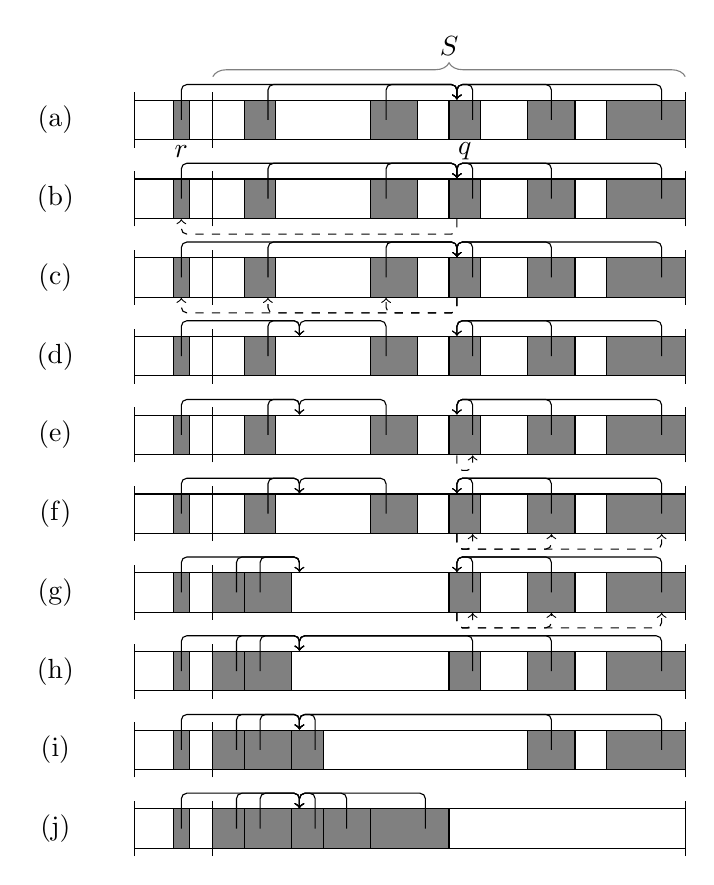
\begin{tikzpicture}
    %% (j)
    \draw (0,0.25) node {(j)};
    \draw (1,0) rectangle (8,0.5);
    \draw (1,-0.1) -- (1,0.6);
    \draw (2,-0.1) -- (2,0.6);
    \draw (8,-0.1) -- (8,0.6);
    \filldraw [fill=gray] (1.5,0) rectangle (1.7,0.5);
    \filldraw [fill=gray] (2,0) rectangle (2.4,0.5);
    \filldraw [fill=gray] (2.4,0) rectangle (3,0.5);
    \filldraw [fill=gray] (3,0) rectangle (3.4,0.5);
    \filldraw [fill=gray] (3.4,0) rectangle (4,0.5);
    \filldraw [fill=gray] (4,0) rectangle (5,0.5);
    \draw [rounded corners=2pt,->] (1.6,0.25) -- (1.6,0.70) -- (3.1,0.70) -- (3.1,0.51);
    \draw [rounded corners=2pt,->] (2.3,0.25) -- (2.3,0.70) -- (3.1,0.70) -- (3.1,0.51);
    \draw [rounded corners=2pt,->] (2.6,0.25) -- (2.6,0.70) -- (3.1,0.70) -- (3.1,0.51);
    \draw [rounded corners=2pt,->] (3.3,0.25) -- (3.3,0.70) -- (3.1,0.70) -- (3.1,0.51);
    \draw [rounded corners=2pt,->] (3.7,0.25) -- (3.7,0.70) -- (3.1,0.70) -- (3.1,0.51);
    \draw [rounded corners=2pt,->] (4.7,0.25) -- (4.7,0.70) -- (3.1,0.70) -- (3.1,0.51);
    %% (i)
    \draw (0,1.25) node {(i)};
    \draw (1,1) rectangle (8,1.5);
    \draw (1,0.9) -- (1,1.6);
    \draw (2,0.9) -- (2,1.6);
    \draw (8,0.9) -- (8,1.6);
    \filldraw [fill=gray] (1.5,1) rectangle (1.7,1.5);
    \filldraw [fill=gray] (2,1) rectangle (2.4,1.5);
    \filldraw [fill=gray] (2.4,1) rectangle (3,1.5);
    \filldraw [fill=gray] (3,1) rectangle (3.4,1.5);
    \filldraw [fill=gray] (6,1) rectangle (6.6,1.5);
    \filldraw [fill=gray] (7,1) rectangle (8,1.5);
    \draw [rounded corners=2pt,->] (1.6,1.25) -- (1.6,1.70) -- (3.1,1.70) -- (3.1,1.51);
    \draw [rounded corners=2pt,->] (2.3,1.25) -- (2.3,1.70) -- (3.1,1.70) -- (3.1,1.51);
    \draw [rounded corners=2pt,->] (2.6,1.25) -- (2.6,1.70) -- (3.1,1.70) -- (3.1,1.51);
    \draw [rounded corners=2pt,->] (3.3,1.25) -- (3.3,1.70) -- (3.1,1.70) -- (3.1,1.51);
    \draw [rounded corners=2pt,->] (6.3,1.25) -- (6.3,1.70) -- (3.1,1.70) -- (3.1,1.51);
    \draw [rounded corners=2pt,->] (7.7,1.25) -- (7.7,1.70) -- (3.1,1.70) -- (3.1,1.51);
    %% (h)
    \draw (0,2.25) node {(h)};
    \draw (1,2) rectangle (8,2.5);
    \draw (1,1.9) -- (1,2.6);
    \draw (2,1.9) -- (2,2.6);
    \draw (8,1.9) -- (8,2.6);
    \filldraw [fill=gray] (1.5,2) rectangle (1.7,2.5);
    \filldraw [fill=gray] (2,2) rectangle (2.4,2.5);
    \filldraw [fill=gray] (2.4,2) rectangle (3,2.5);
    \filldraw [fill=gray] (5,2) rectangle (5.4,2.5);
    \filldraw [fill=gray] (6,2) rectangle (6.6,2.5);
    \filldraw [fill=gray] (7,2) rectangle (8,2.5);
    \draw [rounded corners=2pt,->] (1.6,2.25) -- (1.6,2.70) -- (3.1,2.70) -- (3.1,2.51);
    \draw [rounded corners=2pt,->] (2.3,2.25) -- (2.3,2.70) -- (3.1,2.70) -- (3.1,2.51);
    \draw [rounded corners=2pt,->] (2.6,2.25) -- (2.6,2.70) -- (3.1,2.70) -- (3.1,2.51);
    \draw [rounded corners=2pt,->] (5.3,2.25) -- (5.3,2.70) -- (3.1,2.70) -- (3.1,2.51);
    \draw [rounded corners=2pt,->] (6.3,2.25) -- (6.3,2.70) -- (3.1,2.70) -- (3.1,2.51);
    \draw [rounded corners=2pt,->] (7.7,2.25) -- (7.7,2.70) -- (3.1,2.70) -- (3.1,2.51);
    %% (g)
    \draw (0,3.25) node {(g)};
    \draw (1,3) rectangle (8,3.5);
    \draw (1,2.9) -- (1,3.6);
    \draw (2,2.9) -- (2,3.6);
    \draw (8,2.9) -- (8,3.6);
    \filldraw [fill=gray] (1.5,3) rectangle (1.7,3.5);
    \filldraw [fill=gray] (2,3) rectangle (2.4,3.5);
    \filldraw [fill=gray] (2.4,3) rectangle (3,3.5);
    \filldraw [fill=gray] (5,3) rectangle (5.4,3.5);
    \filldraw [fill=gray] (6,3) rectangle (6.6,3.5);
    \filldraw [fill=gray] (7,3) rectangle (8,3.5);
    \draw [rounded corners=2pt,->] (1.6,3.25) -- (1.6,3.70) -- (3.1,3.70) -- (3.1,3.51);
    \draw [rounded corners=2pt,->] (2.3,3.25) -- (2.3,3.70) -- (3.1,3.70) -- (3.1,3.51);
    \draw [rounded corners=2pt,->] (2.6,3.25) -- (2.6,3.70) -- (3.1,3.70) -- (3.1,3.51);
    \draw [rounded corners=2pt,->] (5.3,3.25) -- (5.3,3.70) -- (5.1,3.70) -- (5.1,3.51);
    \draw [rounded corners=2pt,->] (6.3,3.25) -- (6.3,3.70) -- (5.1,3.70) -- (5.1,3.51);
    \draw [rounded corners=2pt,->] (7.7,3.25) -- (7.7,3.70) -- (5.1,3.70) -- (5.1,3.51);
    \draw [rounded corners=2pt,dashed,->] (5.1,2.99) -- (5.1,2.8) -- (5.3,2.8) -- (5.3,2.99);
    \draw [rounded corners=2pt,dashed,->] (5.1,2.99) -- (5.1,2.8) -- (6.3,2.8) -- (6.3,2.99);
    \draw [rounded corners=2pt,dashed,->] (5.1,2.99) -- (5.1,2.8) -- (7.7,2.8) -- (7.7,2.99);
    %% (f)
    \draw (0,4.25) node {(f)};
    \draw (1,4) rectangle (8,4.5);
    \draw (1,3.9) -- (1,4.6);
    \draw (2,3.9) -- (2,4.6);
    \draw (8,3.9) -- (8,4.6);
    \filldraw [fill=gray] (1.5,4) rectangle (1.7,4.5);
    \filldraw [fill=gray] (2.4,4) rectangle (2.8,4.5);
    \filldraw [fill=gray] (4,4) rectangle (4.6,4.5);
    \filldraw [fill=gray] (5,4) rectangle (5.4,4.5);
    \filldraw [fill=gray] (6,4) rectangle (6.6,4.5);
    \filldraw [fill=gray] (7,4) rectangle (8,4.5);
    \draw [rounded corners=2pt,->] (1.6,4.25) -- (1.6,4.70) -- (3.1,4.70) -- (3.1,4.51);
    \draw [rounded corners=2pt,->] (2.7,4.25) -- (2.7,4.70) -- (3.1,4.70) -- (3.1,4.51);
    \draw [rounded corners=2pt,->] (4.2,4.25) -- (4.2,4.70) -- (3.1,4.70) -- (3.1,4.51);
    \draw [rounded corners=2pt,->] (5.3,4.25) -- (5.3,4.70) -- (5.1,4.70) -- (5.1,4.51);
    \draw [rounded corners=2pt,->] (6.3,4.25) -- (6.3,4.70) -- (5.1,4.70) -- (5.1,4.51);
    \draw [rounded corners=2pt,->] (7.7,4.25) -- (7.7,4.70) -- (5.1,4.70) -- (5.1,4.51);
    \draw [rounded corners=2pt,dashed,->] (5.1,3.99) -- (5.1,3.8) -- (5.3,3.8) -- (5.3,3.99);
    \draw [rounded corners=2pt,dashed,->] (5.1,3.99) -- (5.1,3.8) -- (6.3,3.8) -- (6.3,3.99);
    \draw [rounded corners=2pt,dashed,->] (5.1,3.99) -- (5.1,3.8) -- (7.7,3.8) -- (7.7,3.99);
    %% (e)
    \draw (0,5.25) node {(e)};
    \draw (1,5) rectangle (8,5.5);
    \draw (1,4.9) -- (1,5.6);
    \draw (2,4.9) -- (2,5.6);
    \draw (8,4.9) -- (8,5.6);
    \filldraw [fill=gray] (1.5,5) rectangle (1.7,5.5);
    \filldraw [fill=gray] (2.4,5) rectangle (2.8,5.5);
    \filldraw [fill=gray] (4,5) rectangle (4.6,5.5);
    \filldraw [fill=gray] (5,5) rectangle (5.4,5.5);
    \filldraw [fill=gray] (6,5) rectangle (6.6,5.5);
    \filldraw [fill=gray] (7,5) rectangle (8,5.5);
    \draw [rounded corners=2pt,->] (1.6,5.25) -- (1.6,5.70) -- (3.1,5.70) -- (3.1,5.51);
    \draw [rounded corners=2pt,->] (2.7,5.25) -- (2.7,5.70) -- (3.1,5.70) -- (3.1,5.51);
    \draw [rounded corners=2pt,->] (4.2,5.25) -- (4.2,5.70) -- (3.1,5.70) -- (3.1,5.51);
    \draw [rounded corners=2pt,->] (5.3,5.25) -- (5.3,5.70) -- (5.1,5.70) -- (5.1,5.51);
    \draw [rounded corners=2pt,->] (6.3,5.25) -- (6.3,5.70) -- (5.1,5.70) -- (5.1,5.51);
    \draw [rounded corners=2pt,->] (7.7,5.25) -- (7.7,5.70) -- (5.1,5.70) -- (5.1,5.51);
    \draw [rounded corners=2pt,dashed,->] (5.1,4.99) -- (5.1,4.8) -- (5.3,4.8) -- (5.3,4.99);
    %% (d)
    \draw (0,6.25) node {(d)};
    \draw (1,6) rectangle (8,6.5);
    \draw (1,5.9) -- (1,6.6);
    \draw (2,5.9) -- (2,6.6);
    \draw (8,5.9) -- (8,6.6);
    \filldraw [fill=gray] (1.5,6) rectangle (1.7,6.5);
    \filldraw [fill=gray] (2.4,6) rectangle (2.8,6.5);
    \filldraw [fill=gray] (4,6) rectangle (4.6,6.5);
    \filldraw [fill=gray] (5,6) rectangle (5.4,6.5);
    \filldraw [fill=gray] (6,6) rectangle (6.6,6.5);
    \filldraw [fill=gray] (7,6) rectangle (8,6.5);
    \draw [rounded corners=2pt,->] (1.6,6.25) -- (1.6,6.70) -- (3.1,6.70) -- (3.1,6.51);
    \draw [rounded corners=2pt,->] (2.7,6.25) -- (2.7,6.70) -- (3.1,6.70) -- (3.1,6.51);
    \draw [rounded corners=2pt,->] (4.2,6.25) -- (4.2,6.70) -- (3.1,6.70) -- (3.1,6.51);
    \draw [rounded corners=2pt,->] (5.3,6.25) -- (5.3,6.70) -- (5.1,6.70) -- (5.1,6.51);
    \draw [rounded corners=2pt,->] (6.3,6.25) -- (6.3,6.70) -- (5.1,6.70) -- (5.1,6.51);
    \draw [rounded corners=2pt,->] (7.7,6.25) -- (7.7,6.70) -- (5.1,6.70) -- (5.1,6.51);
    %% (c)
    \draw (0,7.25) node {(c)};
    \draw (1,7) rectangle (8,7.5);
    \draw (1,6.9) -- (1,7.6);
    \draw (2,6.9) -- (2,7.6);
    \draw (8,6.9) -- (8,7.6);
    \filldraw [fill=gray] (1.5,7) rectangle (1.7,7.5);
    \filldraw [fill=gray] (2.4,7) rectangle (2.8,7.5);
    \filldraw [fill=gray] (4,7) rectangle (4.6,7.5);
    \filldraw [fill=gray] (5,7) rectangle (5.4,7.5);
    \filldraw [fill=gray] (6,7) rectangle (6.6,7.5);
    \filldraw [fill=gray] (7,7) rectangle (8,7.5);
    \draw [rounded corners=2pt,->] (1.6,7.25) -- (1.6,7.70) -- (5.1,7.70) -- (5.1,7.51);
    \draw [rounded corners=2pt,->] (2.7,7.25) -- (2.7,7.70) -- (5.1,7.70) -- (5.1,7.51);
    \draw [rounded corners=2pt,->] (4.2,7.25) -- (4.2,7.70) -- (5.1,7.70) -- (5.1,7.51);
    \draw [rounded corners=2pt,->] (5.3,7.25) -- (5.3,7.70) -- (5.1,7.70) -- (5.1,7.51);
    \draw [rounded corners=2pt,->] (6.3,7.25) -- (6.3,7.70) -- (5.1,7.70) -- (5.1,7.51);
    \draw [rounded corners=2pt,->] (7.7,7.25) -- (7.7,7.70) -- (5.1,7.70) -- (5.1,7.51);
    \draw [rounded corners=2pt,dashed,->] (5.1,6.99) -- (5.1,6.8) -- (4.2,6.8) -- (4.2,6.99);
    \draw [rounded corners=2pt,dashed,->] (5.1,6.99) -- (5.1,6.8) -- (2.7,6.8) -- (2.7,6.99);
    \draw [rounded corners=2pt,dashed,->] (5.1,6.99) -- (5.1,6.8) -- (1.6,6.8) -- (1.6,6.99);
    %% (b)
    \draw (0,8.25) node {(b)};
    \draw (1,8) rectangle (8,8.5);
    \draw (1,7.9) -- (1,8.6);
    \draw (2,7.9) -- (2,8.6);
    \draw (8,7.9) -- (8,8.6);
    \filldraw [fill=gray] (1.5,8) rectangle (1.7,8.5);
    \filldraw [fill=gray] (2.4,8) rectangle (2.8,8.5);
    \filldraw [fill=gray] (4,8) rectangle (4.6,8.5);
    \filldraw [fill=gray] (5,8) rectangle (5.4,8.5);
    \filldraw [fill=gray] (6,8) rectangle (6.6,8.5);
    \filldraw [fill=gray] (7,8) rectangle (8,8.5);
    \draw [rounded corners=2pt,->] (1.6,8.25) -- (1.6,8.70) -- (5.1,8.70) -- (5.1,8.51);
    \draw [rounded corners=2pt,->] (2.7,8.25) -- (2.7,8.70) -- (5.1,8.70) -- (5.1,8.51);
    \draw [rounded corners=2pt,->] (4.2,8.25) -- (4.2,8.70) -- (5.1,8.70) -- (5.1,8.51);
    \draw [rounded corners=2pt,->] (5.3,8.25) -- (5.3,8.70) -- (5.1,8.70) -- (5.1,8.51);
    \draw [rounded corners=2pt,->] (6.3,8.25) -- (6.3,8.70) -- (5.1,8.70) -- (5.1,8.51);
    \draw [rounded corners=2pt,->] (7.7,8.25) -- (7.7,8.70) -- (5.1,8.70) -- (5.1,8.51);
    \draw [rounded corners=2pt,dashed,->] (5.1,7.99) -- (5.1,7.8) -- (1.6,7.8) -- (1.6,7.99);
    %% (a)
    \draw (0,9.25) node {(a)};
    \draw (1,9) rectangle (8,9.5);
    \draw (1,8.9) -- (1,9.6);
    \draw (2,8.9) -- (2,9.6);
    \draw (8,8.9) -- (8,9.6);
    \filldraw [fill=gray] (1.5,9) rectangle (1.7,9.5);
    \draw (1.6,8.85) node {$r$};
    \filldraw [fill=gray] (2.4,9) rectangle (2.8,9.5);
    \filldraw [fill=gray] (4,9) rectangle (4.6,9.5);
    \filldraw [fill=gray] (5,9) rectangle (5.4,9.5);
    \draw (5.2,8.85) node {$q$};
    \filldraw [fill=gray] (6,9) rectangle (6.6,9.5);
    \filldraw [fill=gray] (7,9) rectangle (8,9.5);
    \draw [rounded corners=2pt,->] (1.6,9.25) -- (1.6,9.70) -- (5.1,9.70) -- (5.1,9.51);
    \draw [rounded corners=2pt,->] (2.7,9.25) -- (2.7,9.70) -- (5.1,9.70) -- (5.1,9.51);
    \draw [rounded corners=2pt,->] (4.2,9.25) -- (4.2,9.70) -- (5.1,9.70) -- (5.1,9.51);
    \draw [rounded corners=2pt,->] (5.3,9.25) -- (5.3,9.70) -- (5.1,9.70) -- (5.1,9.51);
    \draw [rounded corners=2pt,->] (6.3,9.25) -- (6.3,9.70) -- (5.1,9.70) -- (5.1,9.51);
    \draw [rounded corners=2pt,->] (7.7,9.25) -- (7.7,9.70) -- (5.1,9.70) -- (5.1,9.51);
    %% brace
    \draw [gray,decorate,decoration={brace,amplitude=5pt}] (2,9.8) -- (8,9.8) node [black,midway,above=4pt] {$S$};
  \end{tikzpicture}
  \caption{Example run of Jonkers' algorithm}
  \label{fig:jonkersex}
\end{figure*}

We first describe the algorithm informally and illustrate it by the example given in \cite{Jonkers79}.
The initial situation is given in Fig.~\ref{fig:jonkersex}(a), where only the pointers to an
single node $q$ are shown.

The algorithm starts by visiting the cells in the root set $r_1,\ldots,r_n$. For each root cell $r$
containing a pointer to a node $q$, $r$ cannot be updated immediately since the new address of
the node is not yet known. Therefore $r$ is \emph{threaded} to $q$. For now it does not matter how
this threading is achieved. We will discuss that later.

Fig.~\ref{fig:jonkersex}(b) shows the situation once all cells in the root set have been visisted
this way, where the dashed arrow indicates the \emph{is threaded to} relation. The algorithm continues
by scanning the store $S$ twice, visiting all pointer cells of all nodes in the order from lower
addresses to higher addresses. Upon visiting a node $q$ in the first scan (Fig.~\ref{fig:jonkersex}(c)),
the address where $q$ is to be moved to is known from an accumulated counter. Using this information
all pointer cells threaded to $q$ at this point are updated as shown in Fig.~\ref{fig:jonkersex}(d),
where \emph{updating} a cell also means \emph{unthreading} it.

Subsequently all pointer cells of $q$ containing a pointer to a node are threaded to that node
(Fig.~\ref{fig:jonkersex}(e)). Once the first scan is done all pointer cells in the root set
will have been updated this way. Furthermore, all pointer cells pointing \emph{forward} to
$q$ -- in ascending address order -- will have been updated as well, and all pointer cells
pointing \emph{backward} to $q$, including pointer cells of $q$ itself, will be threaded to
$q$ (Fig.~\ref{fig:jonkersex}(f)).

The second scan visits all nodes in ascending address order again. Upon visiting a node
$q$ (Fig.~\ref{fig:jonkersex}(g)), all pointer cells threaded to $q$ must be backward pointers,
and neither $q$ nor any pointer cell threaded to $q$ will have been moved yet. Therefore all
cells threaded to $q$ can be correctly updated to the new address of $q$ as shown in
Fig.~\ref{fig:jonkersex}(h). Once this is done, all cells pointing to the initial address of
$q$ will have been updated to the new address of $q$, and all nodes to the left of $q$ will
have been moved to their new locations already. Therefore it is now safe to move $q$ to
its new location (Fig.~\ref{fig:jonkersex}(i)) as well. Once the second scan is complete, all
nodes will have been moved and all pointers will have been updated (Fig.~\ref{fig:jonkersex}(j)).

\begin{figure}[htb]
  \centering
  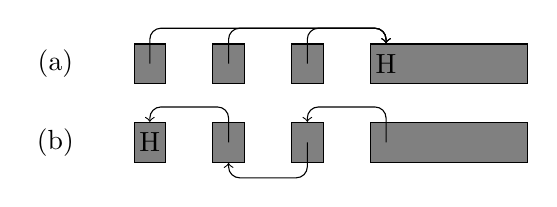
\begin{tikzpicture}
    \draw (0,1.25) node {(a)};
    \filldraw [fill=gray] (1,1) rectangle (1.4,1.5);
    \filldraw [fill=gray] (2,1) rectangle (2.4,1.5);
    \filldraw [fill=gray] (3,1) rectangle (3.4,1.5);
    \filldraw [fill=gray] (4,1) rectangle (6.0,1.5);
    \draw [rounded corners,->] (1.2,1.25) -- (1.2,1.7) -- (4.2,1.7) -- (4.2,1.51);
    \draw [rounded corners,->] (2.2,1.25) -- (2.2,1.7) -- (4.2,1.7) -- (4.2,1.51);
    \draw [rounded corners,->] (3.2,1.25) -- (3.2,1.7) -- (4.2,1.7) -- (4.2,1.51);
    \draw (4.2,1.25) node {H};
    \draw (0,0.25) node {(b)};
    \filldraw [fill=gray] (1,0) rectangle (1.4,0.5);
    \filldraw [fill=gray] (2,0) rectangle (2.4,0.5);
    \filldraw [fill=gray] (3,0) rectangle (3.4,0.5);
    \filldraw [fill=gray] (4,0) rectangle (6.0,0.5);
    \draw [rounded corners,->] (4.2,0.25) -- (4.2,0.7) -- (3.2,0.7) -- (3.2,0.51);
    \draw [rounded corners,->] (3.2,0.25) -- (3.2,-0.2) -- (2.2,-0.2) -- (2.2,-0.01);
    \draw [rounded corners,->] (2.2,0.25) -- (2.2,0.7) -- (1.2,0.7) -- (1.2,0.51);
    \draw (1.2,0.25) node {H};
  \end{tikzpicture}
  \caption{Example of threading}
  \label{fig:threadingex}
\end{figure}

In order to fully understand the algorithm, we have to explain how \emph{threading} works
in detail, especially why this threading of cells can be done without any space overhead
using the well-known trick described in \cite{Fisher74}. By assumption and from the (informal)
description above we know two things:
\begin{enumerate}
\item The first cell of a node contains the header, which is distinguishable from any address.
\item All pointer cells threaded to a node initially contain a pointer to that node.
\end{enumerate}
Now consider the situation shown in Fig.~\ref{fig:threadingex}(a) with 3 cells holding pointers
to a node. We can transform this situation in such a way that all cells threaded to a node
are chained in a list, using the header cell of the node as list head and the original content
of the header cell as list terminator (Fig.~\ref{fig:threadingex}(b)). This transformation can
be performed without loss of information, since both the original content of the header cell
as well as all information about the cells pointing to it is preserved within the structure of
the list.

Updating all cells threaded to a node is now a matter of traversing this list, updating the 
cells in it and restoring the header value of the node using the list terminator. It is
especially important to restore the original header value while scanning a node, since it
may be necessary to determine the size of the node as well as its pointer cells (during the
first scan) or to move the node (during the second scan).

\begin{algorithm}[htb!]
  \caption{Jonkers' garbage compactor}
  \label{alg:jonkers}
  {\footnotesize\begin{algorithmic}[0]
    \Procedure{Thread}{$p$}
      \If{$M[p] \ne \mathbf{nil}$}
        \State $q \gets M[p]; M[p] \gets M[q]; M[q] \gets p$
      \EndIf
    \EndProcedure
    \\
    \Procedure{Scan}{$p$}
      \State $\mbox{let $p_1,\ldots,p_n$ be the addresses of the}$
      \State $\mbox{pointer cells of the node with address $p$}$;
      \For{$i \gets 1,\ldots,n$}
        \State $\Call{Thread}{p_i}$
      \EndFor
    \EndProcedure
    \\
    \Procedure{Update}{$old,new$}
      \State $p \gets M[old]$
      \While{$\Call{IsAddress}{p}$}
        \State $q \gets M[p]; M[p] \gets new; p \gets q$
      \EndWhile
      \State $M[old] \gets p$
    \EndProcedure
    \\
    \Procedure{Move}{$old,new$}
      \For{$i = 0,\ldots,\Call{Size}{old} - 1$}
        \State $M[new + i] \gets M[old + i]$
      \EndFor
    \EndProcedure
    \\
    \Procedure{Compact}{$ $}
      \For{$i \gets 1,\ldots,n$} %\Comment{Thread pointers in the root set}
        \State $\Call{Thread}{r_i}$
      \EndFor
      \State $new \gets s_1$ %\Comment{First pass}
      \For{$i \gets 1,\ldots,m$}
        \State $\Call{Update}{l_i,new};\Call{Scan}{l_i}$
        \State $new \gets new + \Call{Size}{l_i}$
      \EndFor
      \State $new \gets s_1$ %\Comment{Second pass}
      \For{$i \gets 1,\ldots,m$}
        \State $\Call{Update}{l_i,new};\Call{Move}{l_i,new}$
        \State $new \gets new + \Call{Size}{l_i}$
      \EndFor
    \EndProcedure
  \end{algorithmic}}
\end{algorithm}

The whole procedure is described formally in Algorithm~\ref{alg:jonkers} using pseudocode.


\section{Our algorithm}
\label{sec:our}


Jonkers' original algorithm -- as described in the previous section -- does not work if pointers
are allowed to point not only to header addresses but also to interior header addresses. This is because
interior headers are ignored by the \textsc{Update} procedure. If there would be a way to reliably
locate all interior headers of a node, fixing this shortcoming would be a matter of adjusting the
\textsc{Update} procedure to also update pointer cells threaded to the interior headers.
However it may not be feasible, indeed it may even be impossible, to implement this in practice.

Instead, we assume that, given a pointer to an interior header, it is possible to determine the
node, and hence the header of the node, to which this interior address belongs. This is a
realistic assumption and might also be necessary for the marking algorithm anyway.

In this section we will present an extension to Jonkers' algorithm, which is able to thread
pointers to interior headers of a node and update them properly to the new address of the
interior header to which the node will be moved. Our extension shares the good properties
of the original algorithm, which means it does not impose any additional space overhead
and requires linear time in practice.
It does however place additional restrictions on the shape of pointers and cells. Furthermore
it assumes that, given the node header and the interior offset, it is possible to reconstruct
an interior header.

\begin{figure}[htb]
  \centering
  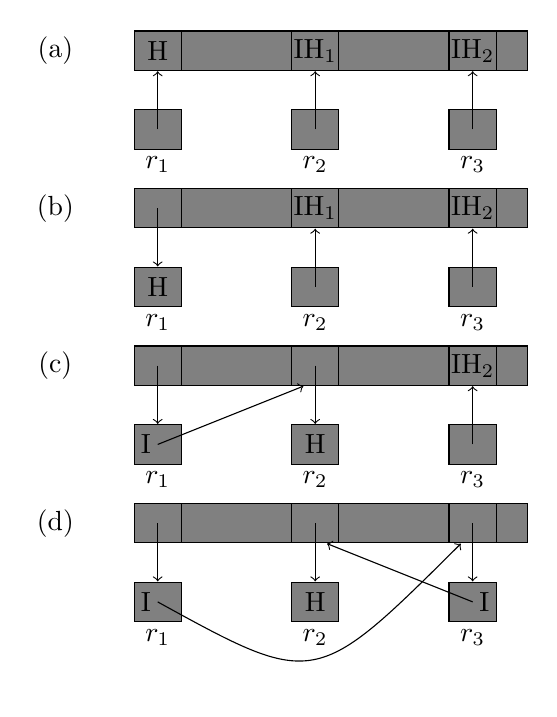
\begin{tikzpicture}
    %% (a)
    \draw (0,9.25) node {(a)};
    \filldraw [fill=gray] (1,9) rectangle (6,9.5);
    \filldraw [fill=gray] (1,9) rectangle (1.6,9.5);
    \draw (1.3,9.25) node {H};
    \filldraw [fill=gray] (3,9) rectangle (3.6,9.5);
    \draw (3.3,9.25) node {IH$_1$};
    \filldraw [fill=gray] (5,9) rectangle (5.6,9.5);
    \draw (5.3,9.25) node {IH$_2$};
    \filldraw [fill=gray] (1,8) rectangle (1.6,8.5);
    \draw [->] (1.3,8.25) -- (1.3,8.99);
    \draw (1.3,7.8) node {$r_1$};
    \filldraw [fill=gray] (3,8) rectangle (3.6,8.5);
    \draw [->] (3.3,8.25) -- (3.3,8.99);
    \draw (3.3,7.8) node {$r_2$};
    \filldraw [fill=gray] (5,8) rectangle (5.6,8.5);
    \draw [->] (5.3,8.25) -- (5.3,8.99);
    \draw (5.3,7.8) node {$r_3$};
    %% (b)
    \draw (0,7.25) node {(b)};
    \filldraw [fill=gray] (1,7) rectangle (6,7.5);
    \filldraw [fill=gray] (1,7) rectangle (1.6,7.5);
    \filldraw [fill=gray] (3,7) rectangle (3.6,7.5);
    \draw (3.3,7.25) node {IH$_1$};
    \filldraw [fill=gray] (5,7) rectangle (5.6,7.5);
    \draw (5.3,7.25) node {IH$_2$};
    \filldraw [fill=gray] (1,6) rectangle (1.6,6.5);
    \draw (1.3,6.25) node {H};
    \draw [->] (1.3,7.25) -- (1.3,6.51);
    \draw (1.3,5.8) node {$r_1$};
    \filldraw [fill=gray] (3,6) rectangle (3.6,6.5);
    \draw [->] (3.3,6.25) -- (3.3,6.99);
    \draw (3.3,5.8) node {$r_2$};
    \filldraw [fill=gray] (5,6) rectangle (5.6,6.5);
    \draw [->] (5.3,6.25) -- (5.3,6.99);
    \draw (5.3,5.8) node {$r_3$};
    %% (c)
    \draw (0,5.25) node {(c)};
    \filldraw [fill=gray] (1,5) rectangle (6,5.5);
    \filldraw [fill=gray] (1,5) rectangle (1.6,5.5);
    \filldraw [fill=gray] (3,5) rectangle (3.6,5.5);
    \filldraw [fill=gray] (5,5) rectangle (5.6,5.5);
    \draw (5.3,5.25) node {IH$_2$};
    \filldraw [fill=gray] (1,4) rectangle (1.6,4.5);
    \draw (1.15,4.25) node {I};
    \draw [->] (1.3,5.25) -- (1.3,4.51);
    \draw (1.3,3.8) node {$r_1$};
    \filldraw [fill=gray] (3,4) rectangle (3.6,4.5);
    \draw [->] (1.3,4.25) -- (3.15,4.99);
    \draw (3.3,3.8) node {$r_2$};
    \draw (3.3,4.25) node {H};
    \draw [->] (3.3,5.25) -- (3.3,4.51);
    \filldraw [fill=gray] (5,4) rectangle (5.6,4.5);
    \draw [->] (5.3,4.25) -- (5.3,4.99);
    \draw (5.3,3.8) node {$r_3$};
    %% (d)
    \draw (0,3.25) node {(d)};
    \filldraw [fill=gray] (1,3) rectangle (6,3.5);
    \filldraw [fill=gray] (1,3) rectangle (1.6,3.5);
    \filldraw [fill=gray] (3,3) rectangle (3.6,3.5);
    \filldraw [fill=gray] (5,3) rectangle (5.6,3.5);
    \filldraw [fill=gray] (1,2) rectangle (1.6,2.5);
    \draw (1.3,1.8) node {$r_1$};
    \draw (1.15,2.25) node {I};
    \filldraw [fill=gray] (3,2) rectangle (3.6,2.5);
    \draw (3.3,1.8) node {$r_2$};
    \draw (3.3,2.25) node {H};
    \filldraw [fill=gray] (5,2) rectangle (5.6,2.5);
    \draw (5.3,1.8) node {$r_3$};
    \draw [->] (1.3,3.25) -- (1.3,2.51);
    \draw [->] (1.3,2.25) .. controls (3.3,1.15) .. (5.15,2.99);
    \draw [->] (3.3,3.25) -- (3.3,2.51);
    \draw [->] (5.3,3.25) -- (5.3,2.51);
    \draw [->] (5.3,2.25) -- (3.45,2.99);
    \draw (5.45,2.25) node {I};
  \end{tikzpicture}
  \caption{Example of threading with interior pointers}
  \label{fig:threadinginterior}
\end{figure}

Consider the situation given in Fig.~\ref{fig:threadinginterior}(a) with three pointers $r_1$, $r_2$ and
$r_3$ pointing to a node, where $r_1$ points to the header H of the node while $r_2$ and $r_3$ point to
the interior headers IH$_1$ and IH$_2$ respectively. Upon visiting $r_1$ it can be threaded to the node
as described in the previous section (Fig.~\ref{fig:threadinginterior}(b)).

However the pointer cell $r_2$ cannot simply be threaded to the interior header IH$_1$, since by
assumption we are unable to locate all interior headers of a node, and as such the pointer cells threaded
to an interior header of a node would not be updated.

The basic idea of our algorithm is to thread interior pointer cells to the node header just like
cells pointing to the header of a node. Since the interior pointer cells need special treatment
during update we chain both the interior header cell and the interior pointer cell, while tagging
the pointer to the interior header in special way as shown in Fig.~\ref{fig:threadinginterior}(c).
Once all pointers and interior pointers to a node are threaded, the situation looks as given in
Fig.~\ref{fig:threadinginterior}(d).

\begin{algorithm}[htb!]
  \caption{Threading with interior pointers}
  \label{alg:threadnew}
  {\footnotesize\begin{algorithmic}[0]
    \Procedure{Thread}{$p$}
      \State $q \gets M[p]$
      \If{$\Call{IsInteriorHeader}{M[q]}$}
        \State $o \gets \Call{NodeOfInteriorAddress}{q}$
        \While{$\Call{IsPointer}{M[o]}$}
          \State $o \gets M[o]$
        \EndWhile
        \State $M[p] \gets M[o]$
        \State $M[q] \gets p$
        \State $M[o] \gets \Call{InteriorPointer}{q}$
      \Else
        \State $M[p] \gets M[q]$
        \State $M[q] \gets p$
      \EndIf
    \EndProcedure
    \\
    \Procedure{Update}{$old,new$}
      \State $h \gets M[old]$
      \While{$\mathbf{not}\,\Call{IsHeader}{h}$}
        \State $h \gets M[\Call{Pointer}{h}]$
      \EndWhile
      \State $p \gets M[old]$
      \State $n \gets new$
      \While{$\mathbf{not}\,\Call{IsHeader}{p}$}
        \If{$\Call{IsPointer}{p}$}
          \State $q \gets M[p]$
          \State $M[p] \gets n$
        \Else\Comment{$p$ must be an interior pointer}
          \State $p \gets \Call{Pointer}{p}$
          \State $n \gets new + (p - old)$
          \State $q \gets M[p]$
          \State $M[p] \gets \Call{MakeInteriorHeader}{h, old, p}$
        \EndIf
        \State $p \gets q$
      \EndWhile
      \State $M[old] \gets p$
    \EndProcedure
  \end{algorithmic}}
\end{algorithm}

When updating cells we replace pointers with the $new$ address of the node as described in
Jonkers' algorithm. Upon reaching a tagged pointer we know that the cell pointed to originally
contained an interior header and the remaining cells in the chain (up to the terminating header or up to the
next tagged pointer) originally pointed to this interior header. Therefore we reconstruct
the interior header, store it into the cell pointed to by the tagged pointer, set $new$ to the
address of the interior header at the new location of the node and continue updating the remaining 
cells in the list.

While the original algorithm requires the ability to distinguish header values from addresses, our
algorithm imposes additional constraints. This is because threading now requires the ability to
distinguish headers and interior headers, and updating now requires the ability to distinguish
headers, threaded pointers and pointers to interior header cells. To sum up, we need to distinguish
the following:
\begin{enumerate}
\item Values of node headers
\item Pointers to node headers
\item Values of interior headers
\item Pointers to interior headers
\end{enumerate}
Given that we are able to distinguish the above, we can implement the changes necessary to handle
interior pointers as shown in Algorithm~\ref{alg:threadnew}. The rest of the algorithm remains
unchanged.

It is easy to see that the new algorithm is correct. Cells with pointers to the node header will
be chained to the beginning of the threaded list before any cells with pointers to interior headers.
So these pointers will be updated with the $new$ location of the node.

Cells with pointers to interior headers will always be linked in between the tagged pointer that
contains the address of this interior header and the next tagged pointer that contains the address
of another interior header (or the terminating node header). Furthermore since interior headers
threaded to a node are replaced with pointers, the same interior cell cannot be threaded more than
once. Therefore each interior header cell on the list is updated exactly once and the pointer cells
threaded to it will be updated to the correct interior address at the new location of the node.


\section{Efficiency}
\label{sec:efficiency}


The original algorithm visits every node twice, and performs at most one test, thread and update
operation per pointer cell, and exactly one move per node. This results in a worst-case time
complexity of $O(k + n)$, where $k$ is the number of cells in the store and $n$ is the number
of cells in the root set. Since the root set is usually smaller than the store, Jonkers' algorithm
is said to be linear in the size of the store.

The extended algorithm performs the same operations. However, in contrast to the original algorithm,
\textsc{Thread} has to traverse the list of previously threaded pointer cells once for each interior
header being pointed to. The worst-case time complexity is therefore $O(k \cdot (k + n))$. This seems to
be a major regression compared to the original algorithm upon first sight. However, in practice
the number of interior headers is probably low\footnote{Note that the worst-case time complexity
of the extended algorithm is still $O(k + n)$ in the absence of interior headers.}. Furthermore it
has been observed that most live objects in modern applications have only a single referent
\cite{BlackburnGHKMBDFFGHHJLMPSVDW06,DeutschBobrow76,DieckmannH99,WegielKrintz09}. Hence, within a
realistic application, the \textsc{Thread} procedure requires constant time, and as such, the whole
algorithm is linear in the size of the store.

Moreover, under the assumption that appropriate header and interior header cells are available
for the cells, the extended algorithm requires no space overhead. Since each node usually has to
carry additional information such as size and type of the node content, the runtime environment will
have to reserve space for this kind of information anyway (usually as part of a header word).
Interior headers on the other hand might require some extra effort, and will usually carry
information such as the offset of the interior address relative to the address of the first
cell. This kind of information is often already required by the marking phase of the garbage
collector.

The algorithm as described here leaves some room for performance improvements with respect to effective
garbage collection time. For example, the \textsc{Update} routine as shown in Algorithm~\ref{alg:threadnew}
first traverses the list of threaded cells to determine the original header of the node. This information is
used to reconstruct the interior headers within this block. However, since interior headers
should be rare, it might be better to determine this information only on-demand. In fact, it
might even be possible to get by without this additional list traversal if the reconstruction
algorithm does not need the original node header at all (i.e. if the interior header contains
only the offset of the interior cell relative to the first cell of the node).

The additional requirement to distinguish four different kinds of values is also rather
simple to fullfil in practice. Under the assumption that all words are aligned on 4-byte
address boundaries (which may already be required by the addressing constraints of the
target machine), one can use the two least significant bits of machine words to distinguish
4 different kinds of values.


\section{Related work}
\label{sec:related}


There exists a different class of moving compaction algorithms, which perform pointer adjustments
based on range checks within a \emph{break table} \cite{FitchNorman78,HaddonWaite67,LangWegbreit72,Wegbreit72},
and therefore support interior pointers \emph{out of the box}. However these algorithms
either do not operate in time linear to the size of the store
\cite{FitchNorman78,HaddonWaite67,Wegbreit72}, or require substantial space
overhead \cite{LangWegbreit72,Wegbreit72}.

The algorithm presented in \cite{Morris78} is somewhat similar to the basic algorithm described
in section~\ref{sec:jonkers}, and is capable of updating arbitrary interior pointers. But it is
less efficient than the algorithm described here and requires additional space overhead (one
mark bit per cell).


\section{Conclusions}
\label{sec:conclusion}


We have described an algorithm that extends Jonkers' fast garbage compaction algorithm
with the ability to handle pointers to certain interior cells of live objects without any additional
space overhead. The extended algorithm is linear in the size of the store in practice 
and requires one additional bit per value -- compared with the requirements of the
original algorithm -- to differentiate four kinds of cell values relevant for threading and
updating the pointer cells.


\section*{Acknowledgements}

We would like to thank Kurt Sieber and Christian Uhrhan for their careful proof-reading.


%% References
\bibliographystyle{habbrv}
\bibliography{citations}


\end{document}